\documentclass[12pt,a4paper]{article}
\usepackage[ngerman]{babel}
\usepackage{amsmath}
\usepackage{amsfonts}
\usepackage{amssymb}
\usepackage{graphicx}
\usepackage{url}
\usepackage{alltt}

\usepackage{hyperref}
\usepackage[figure]{hypcap}
\usepackage{pdfpages}
\usepackage{titling}
\usepackage{float}
\usepackage[printonlyused]{acronym}
\usepackage[format=plain,
      justification=RaggedRight,
      singlelinecheck=false]
     {caption}
\usepackage[left=2.5cm,right=2.5cm,top=2.5cm,bottom=3cm]{geometry}
\author{Janik Frick}
\title{Konzipierung und Erstellung eines Parametertabellenkonfigurators und Praxisnahe Mitarbeit\\\vspace{0.35cm}
 im releasten Produkt LC-VISION}
\usepackage{setspace}
\usepackage{scrextend}
\deffootnote[1em]{1em}{1em}{%
   \textsuperscript{\thefootnotemark}%
}
\usepackage{enumitem}
\usepackage{fancyhdr}
\addtolength{\headheight}{1.5cm} % make more space for the header
\pagestyle{fancyplain} % use fancy for all pages except chapter start
\lhead{
\includegraphics[width=50mm,scale=1]{blum-logo.PNG}}
\rhead{
\includegraphics[width=50mm,scale=1]{dhbw.png}}
\renewcommand{\headrulewidth}{0pt} % remove rule below header

\newcommand{\dualerPartner}{Blum-Novotest GmbH, Standort Grünkraut}
\newcommand{\hochschule}{Dualen Hochschule Baden-Württemberg Ravensburg}
\newcommand{\betreuer}{Mallmann, Guilherme, Dr.-Ing.}
\newcommand{\studiengang}{Informatik}
\newcommand{\kurs}{TIT21, Matrikelnummer 4268671}
\pagenumbering{arabic}

\begin{document}
\begin{titlepage}

\includegraphics[width=50mm,scale=1]{blum-logo.PNG}
\hfill

\includegraphics[width=50mm,scale=1]{dhbw.png}
   \begin{center}
       \textbf{\huge{\thetitle}}\\
       \vspace{2cm}
       \Large{Projektarbeit T1000\\
       des Studiengangs \studiengang\\
       an der \hochschule\\
       \vspace{1.5cm}
       von\\
       \vspace{0.5cm}
       \theauthor}
       
   \end{center}
       \vspace{1.6cm}
       \noindent
       \vspace{0.3cm}
       \textbf{\large{Kurs: \kurs}}\\
       \vspace{0.3cm}
       \textbf{\large{Dualer Partner: \dualerPartner}}\\
       \vspace{0.3cm}
       \textbf{\large{Betreuer: \betreuer}}
       

\end{titlepage}
\thispagestyle{empty}

\noindent\fbox{%
    \parbox{\textwidth}{%\\
{\large \textbf{Erklärung}}\\\newline\noindent    
gemäß Ziffer 1.1.13 der Anlage 1 zu §§ 3, 4 und 5  der Studien- und Prüfungsordnung für die Bachelorstudiengänge im Studienbereich Technik der Dualen Hochschule Baden-Württemberg vom 29.09.2017.\\Ich versichere hiermit, dass ich meine Projektarbeit mit dem Thema: Konzipierung und Erstellung eines Parametertabellenkonfigurators und Praxisnahe Mitarbeit
 im releasten Produkt LC-VISION selbstständig verfasst und keine anderen als die angegebenen Quellen und Hilfsmittel benutzt habe. Ich versichere zudem, dass die eingereichte elektronische Fassung
mit der gedruckten Fassung übereinstimmt.
\vspace{1cm}\\
Janik Frick
\vspace{1.5cm}\\--------------------------------------------------\hfill -----------------------------------\\
Ort, Datum \hfill Unterschrift
    }%
}
\vspace{1.5cm}\\\fbox{%
    \parbox{\textwidth}{% 
    {\Large \textbf{Sperrvermerk}}\\
\\
\newline
gemäß Ziffer 1.1.13 der Anlage 1 zu §§ 3, 4 und 5  der Studien- und Prüfungsordnung für die Bachelorstudiengänge im Studienbereich Technik der Dualen Hochschule Baden-Württemberg vom 29.09.2017:
\newline
„Der Inhalt dieser Arbeit darf weder als Ganzes noch in Auszügen Personen außerhalb des Prüfungsprozesses und des Evaluationsverfahrens zugänglich gemacht werden, sofern keine anders lautende Genehmigung vom Dualen Partner vorliegt.“
\vspace{1cm}\\
Janik Frick
\vspace{1.5cm}\\
--------------------------------------------------\hfill
-----------------------------------\\
Ort, Datum \hfill Unterschrift
}}
\newpage
\tableofcontents
\thispagestyle{empty}
\newpage
\onehalfspacing
\noindent
\thispagestyle{empty}
{\Large Abkürzungsverzeichnis}\\
\newline
\begin{acronym}[Abkürzungsverzeichnis]
\acro{Blum}[Blum]{Blum-Novotest GmbH}
\acro{GUI}[GUI]{Grafische Benutzeroberfläche}
\acro{MVP}[MVP]{Minimum Viable Product}
\acro{UML}[UML]{Unified Modeling Language}
\end{acronym}
\newpage
\thispagestyle{empty}
\listoffigures
\newpage\setcounter{page}{1}\noindent
{\Large Abstract}\\\newline
\noindent
By developing a \glqq Parametertabellenkonfigurator\grqq\space the dependency on experience of the persons knwoledge about configuring Blum products could be reduced. This is because the description for the current selected parameter is selected by the software and shown in the same window as the file with parameters which is currently worked on. By that the risk of reading the wrong description is eliminated. It also reduces the time in focus, because of less time needed to configure the parameters. These factors lower the risk of errors.\\
By the exmaple of the collaboration on the \glqq LC-VISION\grqq -Software a process of finding orientation in unknown, existing structures is described.\\
\newline
\noindent
{\Large Zusammenfassung}\\
\newline
Mit Hilfe der Entwicklung des \glqq Parametertabellenkonfigurators\grqq kann die Abhängigkeit von der Erfahrung, mit der Erfahrung in der Einrichtung von Produkten von Blum, des Inbetriebnehmers reduziert werden. Die Beschreibungen der einzelnen Parameter werden von der Software automatisch gesucht und im selben Fenster angezeigt, wie die Parametertabelle, die aktuell bearbeitet wird. Diese Automatisierung reduziert das Risiko die falsche Beschreibung zu lesen. Außerdem wird die Zeit, in der die Konzentration gehalten werden muss, reduziert, da die Zeitersparnis bei der Suche nach der richtigen Beschreibung, die Dauer der Konfiguration verkürzt.\\
Am Beispiel der Mitarbeit an der \glqq LC-VISION\grqq -Software wird eine Möglichkeit beschrieben, mit der man Orientierung in unbekannten, schon existierenden Strukturen finden kann.
\noindent

\newpage   
\section{Einleitung}
Die \ac{Blum} ist im Bereich Maschinenbau für Mess- und Prüftechnik tätig.\\
Produkte von \ac{Blum} werden in vielen anspruchsvollen Industrien im Bereich der Qualitätssicherung eingesetzt. Die Kunden kommen unter anderem aus der Automobil-, Luftfahrt- und der Medizinbranche. \\
An die Produkte dieser Industrien werden höchste Qualitätsansprüche gestellt. Daraus resultieren auch für die Produkte der Firma \ac{Blum} höchste Ansprüche. \\
Um diese Ansprüche erfüllen zu können, werden sowohl bestehende Produkte laufend optimiert und weiterentwickelt, als auch neue Produkte entwickelt. \\
Ziel der Arbeit ist es die vielfältigen Aspekte der Softwareentwicklung kennenzulernen und einen Einstieg zu finden.\\
Um dieses Ziel zu erreichen, besteht die Arbeit aus drei Teilen. Im ersten Teil wird ein allgemeiner Überblick über das Vorgehen und die Schritte der Softwareentwicklung gegeben. Im zweiten Teil sollen mit der Entwicklung eines \glqq Parametertabellenkonfigurators\grqq\space die verschiedenen Aufgaben der Softwareentwicklung an einem praktischen Beispiel veranschaulicht werden.
Durch die Mitarbeit am schon bestehenden Produkt \glqq LC-VISION\grqq\space wird das Einarbeiten in unbekannte Strukturen thematisiert. 
\newpage   
% !TEX root = 4268671_Janik_Frick_T1000.tex
\section{Softwareentwicklung}
Das Schreiben von Code ist nur einer von vielen Teilen der Softwareentwicklung. Das Erfassen des Problems, das Design und die Produktpflege sind ebenfalls Teil der Softwareentwicklung\cite{blackwell2002programming}. Der Prozess beginnt mit der Anforderungsanalyse. Auf Basis der Anforderungen wird ein Grobentwurf entwickelt, der als Grundlage für die Implementierung dient. Der Prozess endet mit der Produktpflege und dem Service für das Produkt.
\subsection{Anforderungsanalyse}
Eindeutige und präzise Anforderungen bilden die Grundlage für ein funktionierendes Projekt\cite{doi:10.1080/12460125.2016.1187390}.
Daraus folgt, dass es nicht ausreichend ist, die Liste der Anforderungen zu lesen. Anforderungen müssen analysiert und mit weiterem Wissen über das Projektumfeld kombiniert werden. \\
Dafür gibt es mehrere Techniken, die eingesetzt werden können. 
\subsubsection{Interviews}
\label{interview}
Interviews bieten die Möglichkeit in direkten Gesprächen mit Personen aus dem Umfeld des Projekts Informationen zu sammeln. Diese Informationen können Risiken sein, die zu berücksichtigen sind, Schwierigkeiten bei der aktuellen Vorgehensweise, sowie Abläufe die beibehalten werden sollten.\\
Der Erfolg dieser Vorgehensweise hängt dabei von allen beteiligten Personen ab. Fehlt Wissen über das Umfeld des Projekts kann es zu Schwierigkeiten beim Sammeln der Fragen kommen, wodurch manche Aspekte nicht berücksichtigt werden. Auch die Befragten können Probleme haben ihre Gedanken und ihr Wissen wiederzugeben \cite{tiwari2012selecting}. Das kann die Auswertung der Antworten erschweren.
\subsubsection{Fragebögen}
\label{Fragebögen}
Fragebögen geben den befragten Personen die Möglichkeit ohne direkte Beeinflussung durch den Ersteller der Fragen, Informationen bereitzustellen. Zusätzlich reduzieren sie den Zeitdruck unter dem geantwortet werden soll und alle Befragten antworten auf die gleiche Fragestellung.\\
Fragebögen können eingesetzt werden um Annahmen zu bestätigen oder nach Meinungen und Vorschlägen zu fragen\cite{tiwari2012selecting}. \\
Bei Einsatz dieser Methode ist darauf zu achten die Fragen offen zu formulieren, um die Antworten nicht in eine Richtung zu lenken. 
\subsubsection{Beobachtung}
\label{Beobachtung}
Die Beobachtungsmethode dient dazu aus beobachteten Vorgängen Informationen zu sammeln. \\
Diese Beobachtung kann offen oder verdeckt durchgeführt werden. Bei der verdeckten Vorgehensweise ist das beobachtete Verhalten natürlicher und realistischer, als bei der offenen Vorgehensweise\cite{silhavy2011requirements}. \\
Mit diesem Vorgehen lassen sich Abläufe bei Aufgaben nachvollziehen. Gründe für dieses Abläufe sollten durch andere Techniken in Erfahrung gebracht werden.\\
\subsubsection{Anforderungstypen}
\label{Anforderungstypen}
Anforderungen können in zwei Typen unterteilt werden: Die funktionalen und die nicht funktionalen Anforderungen. Dabei ist zu beachten, dass keine eindeutige Trennung zwischen den beiden Anforderungstypen sinnvoll ist, wie die Ergebnisse der Untersuchung von Eckhardt et al. zeigen\cite{10.1145/2884781.2884788}.
\\Funktionale Anforderungen geben vor, für welche Aufgaben das Produkt geplant wird und welche Funktionen dafür benötigt werden. Die Validierung dieser Anforderungen ist gegeben, da am Ende eindeutig ist, ob eine Funktionalität verfügbar ist. \\
Die nicht funktionalen Anforderungen geben vor, mit welchem Vorgehen und welchen Tools eine Funktion umgesetzt werden soll\cite{10.1145/2884781.2884788}. \\
Auch Anforderungen für Performance wie beispielsweise Reaktionszeiten, vorgegebene Schnittstellen zu anderer Software, wie dem Betriebssystem, können Teil der nicht funktionalen Anforderungen\cite{10.1145/2884781.2884788}. 
Die gegebenen Beispiele sind keine vollständige Aufzählung, da es sehr viele Bereiche gibt, aus denen nicht funktionale Anforderungen stammen können.
Nicht funktionale Anforderungen sind häufig unpräzise formuliert und somit problematisch in der Validierung\cite{10.1145/2884781.2884788}.
\subsection{Dokumentation}
\label{Dokumenation}
Die Dokumentation von Softwareprojekten ist neben der eigentlichen Entwicklung ein relevanter Teilaspekt. Die Dokumentation dient zur Sicherung von Wissen und Grundlagen von Entscheidungen. \\
Die Dokumentation kann in zwei Bereiche unterteilt werden. Die Dokumentation des Codes und die Dokumentation für den Anwender\cite{THEUNISSEN2022106733}.\\
\subsubsection{Sourcecode-Dokumentation}
Diese Form der Dokumentation soll Wissen über die Software beinhalten. Dazu zählen Grundlagen für Entscheidungen der Softwarearchitektur und die Aufgaben von Funktionen, Methoden und Variablen.\\
Die Relevanz besteht darin Wissensverlust zu verhindern, der entsteht, wenn der Entwickler nicht zur Verfügung steht. Dieser Verlust beeinflusst die Einarbeitungsdauer eines neuen Mitarbeiters und somit auch die Produktpflege. \\
Diese Problematik der mangelnden Softwaredokumentation ist in agilen Umfeldern bekannt. Sich ändernde Anforderungen verursachen die Notwendigkeit die Software anzupassen, was Anpassungen der Dokumentation erfordert. Geänderte Anforderungen bringen auch neue kurzfristige Aufgaben mit sich, denen eine höhere Priorität beigemessen wird, als der Aktualisierung der Dokumentation. Kommen viele Änderungen in kurzer Zeit stauen sich die anstehenden Änderungen auf und sorgen für einen hohen Zeitaufwand der Dokumentation. Dies resultiert oftmals in einer vernachlässigten Dokumentation.\\
Weitere potenzielle Schwierigkeiten resultieren aus der Ansicht, dass der Code bereits eine ausreichende Dokumentation für diesen Zweck darstellt und dass Informationen häufig informell und verbal kommuniziert werden, was dazu führen kann, dass diese Informationen nach der Verarbeitung nirgends festgehalten sind und dadurch verloren gehen können\cite{THEUNISSEN2022106733}.\newline
\noindent
\subsubsection{User-Dokumentation}
Der Dokumentation für die Anwender, Servicepersonal und Support-Mitarbeiter wird meist mehr Bedeutung beigemessen, da sie für den Einsatz des Produktes relevant ist.\\
Diese Dokumentation beinhaltet Fehlermeldungen, Voraussetzungen für die Installation und Informationen für die Verwendung. Probleme mit dieser Dokumentation können Schwierigkeiten im Kundenservice verursachen. Probleme dieser Art können einen direkten Einfluss auf den Erfolg eines Produktes oder der Firma haben. Diese möglichen Konsequenzen sorgen dafür, dass dieser Dokumentation mehr Bedeutung beigemessen wird\cite{THEUNISSEN2022106733}.

\subsection{Grobentwurf}
Beim Grobentwurf werden die Hauptbestandteile der Software und die Softwarearchitektur geplant. Dabei sollte der Kunde möglichst miteinbezogen werden, denn der Kunde hat großen Anteil am Gelingen des Projekts\cite{10.1145/1060710.1060712}. \\
Um den Kunden einzubeziehen, können Prototypen eingesetzt werden.\\
Hat das Programm eine \ac{GUI} so kann der Grobentwurf unterschiedlich geplant werden. \\
\subsubsection{GUI mit Bildern}
\label{GUI mit Bildern}
Der Grobentwurf der \ac{GUI} kann mit Hilfe von Bildern in einem beliebigen Bilderstellungsprogramm nachgebildet werden. Die erstellten Entwürfe dienen als Gesprächsgrundlage für eventuell notwendige Veränderungen. Hierbei ist zu beachten, dass die Simulation von Verbindungen zwischen \ac{GUI}-Elementen zeitaufwendig oder gar nicht möglich ist.
\subsubsection{Prototypen}
\label{Prototypen}
Ein Prototyp ist eine funktionierende, begrenzte Version der Anwendung, die als Basis für Gespräche und die Entwicklung weiterer Prototypen dient\cite{budde1992prototyping}. \\
Dieser Prototyp kann durch Software, oder mit einem Mockup-Tool\footnote{Tool um eine \ac{GUI} zu simulieren}, oder auch in einer Software für Präsentationen, realisiert werden. Ein auf Software basierter Prototyp erfordert die Mitarbeit der Entwickler im Design Prozess. 
\subsubsection{User-Tests}
\label{User-Tests}
Bei User Tests wird einer oder mehreren Testpersonen, abhängig von der Verfügbarkeit, der aktuelle Prototyp, siehe \ref{Prototypen}, vorgelegt. Dann kann man der Testperson eine konkrete Aufgabe geben, oder sie den Prototyp frei entdecken lassen. Bei beiden Vorgehensweisen werden Probleme dokumentiert. Stehen mehrere Testpersonen zur Verfügung können auch Gruppentests durchgeführt werden. Bei diesen arbeiten mehrere Personen an einer Aufgabe. Bei Einzel-Tests lassen sich Probleme im Ablauf besser erkennen. In Gruppen-Tests hingegen kann besser nachvollzogen werden, welchen individuellen Problemen Benutzer begegnen\cite{BASTIEN2010e18}. Beide Problemquellen sollten für den Entwurf einer intuitiven Benutzeroberfläche berücksichtigt und möglichst behoben werden. \\
Mit dieser Testmethodik lassen sich nur Prototypen, siehe \ref{Prototypen}, testen, da nur hier die Verbindungen funktional sind.
\subsubsection{30-Sekunden Tests}
\label{30-Sekunden Tests}
Bei 30-Sekunden-Tests bekommen die Testpersonen 30 Sekunden Zeit, um den Prototyp zu erkunden. Nach 30 Sekunden wird ein Fragebogen ausgefüllt, auf dem die Übersichtlichkeit bewertet wird\cite{vsimek2015usability}. \\
30-Sekunden Tests lassen sich mit Bildentwürfen, siehe \ref{GUI mit Bildern}, und mit Prototypen, siehe  \ref{Prototypen}, durchführen, da es bei beiden Entwürfen möglich ist ein Element für 30 Sekunden zu zeigen.
\subsubsection{Heatmaps}
\label{Heatmaps}
Heatmaptools markieren farbig welche Bereiche einer Benutzeroberfläche oft genutzt werden und welche seltene\cite{10.1145/2470654.2466442}. Diese Daten geben Informationen darüber ob Kernfunktionen anders positioniert werden sollten.\\
Diese Methode lässt sich für Bildentwürfe, siehe \ref{GUI mit Bildern}, und Prototypen, siehe \ref{Prototypen}, verwenden.

\subsection{Implementierung}
Der Aufwand der Implementierung lässt sich nicht zwingend aus dem Vorgehen bei der Entwicklung eines Grobentwurfs ableiten. Wurden die Grobentwürfe, wie in \ref{GUI mit Bildern} beschrieben, als einzelne Bilder entworfen, muss zwar von Grund auf neu begonnen werden den Code zu schreiben, es müssen aber auch keine Schwierigkeiten, die durch eine unsaubere Programmierung entstanden sind, gelöst werden. \\
Wird mit Prototypen, (\ref{Prototypen}), gearbeitet, kann dies den Implementierungsprozess beschleunigen. Kommt ein Mockup-Tool zum Einsatz muss die Software ebenfalls von Grund auf programmiert werden, aber der Mock-Up Prototyp dient als Hilfestellung um die Übersicht über die notwendigen Verbindungen zwischen \ac{GUI}-Elementen zu behalten.\\
Programmierte Prototypen bieten zwar die benötigten Funktionalitäten, sind aber nicht zwingend für den praktischen Einsatz geeignet. Ursachen können in unter anderem in fehlender Kompatibilität der Programmiersprache des Prototyps mit dem Zielsystem liegen. Auch wenn die Programmiersprache übereinstimmt kann es sein, dass für den Einsatz als Prototyp für den Grobentwurf externe Abhängigkeiten nicht berücksichtigt werden. Dies kann dazu führen, dass die Integration externer Abhängigkeiten so aufwendig wäre, dass es wirtschaftlicher ist die Implementierung von Grund auf zu beginnen.\\
Entscheidungen was Design und Technologien betrifft, sollten vor Beginn der Implementierung getroffen worden sein. Die Aufgabe der Entwickler besteht darin das geplante Design so in Module zu unterteilen, das es programmiert werden kann\cite{rakos1990software}. 
\subsubsection{Tests}
\label{Tests}
Durch Tests wird validiert, ob die Software die Anforderungen erfüllt. Dabei sollten alle Ergebnisse von Tests dokumentiert werden, um Fehlerquellen, Lösungen und die Kosten für das Beheben der Fehler im Überblick zu behalten\cite{rakos1990software}.\\
Diese bestehen aus mehreren Stufen.
\begin{description}
\item{\underline{Modultests}}\hfill\\
Programmierte Module werden isoliert getestet, um zu prüfen, ob das Modul die Aufgaben erfüllt. Dazu kann auch ein simulierter Input verwenden, wenn benötigte Module noch nicht verfügbar sind. \\
Diese Tests können in zwei Arten unterteilt werden. Bei 'white-box' Tests wird das Modul in einzelnen Schritten getestet. Der Tester weiß wie die Daten verarbeitet werden. Bei 'black-box' Tests versucht der Tester das Vorgehen eines Nutzers nachzustellen. Dabei ist dem Tester die genaue Verarbeitung egal\cite{rakos1990software}.
\item{\underline{Low-Level Integrationstests}}\hfill\\
In diesem Stadium werden die Aufrufe und Rückgabewerte von anderen Modulen getestet. Dabei spielt es keine Rolle, von wem die abhängigen Module entwickelt wurden. Stehen keine realen Daten zur Verfügung kann mit simulierten Daten gearbeitet werden.\cite{rakos1990software}.\\
Ob diese Tests manuell oder automatisiert stattfinden hängt von unterschiedlichen Faktoren ab.
\end{description}
Mit diesem Vorgehen sind alle Module und ihre Abhängigkeiten auf ihre Funktionalität überprüft. Auf dieser Basis wird eine Version erstellt und getestet die in dieser Form praxistauglich ist. Parallel wird daran gearbeitet die benötigten Umgebungsbedingungen bereitzustellen. Dieses Setup wird auf Funktionalität geprüft. Bei erfolgreichem Verlauf der Tests kann die Dokumentation für den Kunden, siehe \ref{Dokumenation}, fertiggestellt werden.
Bestätigt der Kunde das Resultat kann mit dem Training betreuender Personen und Benutzern begonnen werden\cite{rakos1990software}.\\
\subsubsection{Test Automatisierung}
Das manuelle Ausführen von Tests kann zeitaufwändig sein, wodurch man auf die Idee kommen kann diese Tests zu automatisieren. Diese Entscheidung ist dabei von unterschiedlichen Faktoren abhängig. \\
Die Erfahrung des Verantwortlichen beeinflusst die Dauer für die Automatisierung maßgeblich. Auch die Umgebung, in der die Anwendung funktionieren soll, muss automatisiert simuliert werden. Basiert die Funktionalität der Software auf Benutzereingaben, oder läuft sie nach dem Start alleine? Anwendungen die selbstständig ablaufen, sind meistens einfacher zu testen, als solche bei denen man eine automatisierte Benutzerinteraktion nachstellen muss\cite{fewster1999software}. \\
Diese und noch weitere Faktoren beeinflussen den Aufwand für die Automatisierung von Tests. Es muss also eine Kosten-Nutzen-Analyse durchgeführt werden um entscheiden zu können, ob die Automatisierung einen Mehrwert bietet.
\subsection{Objektorientierung}
\label{Objektorientierung}
In der Objektorientierung können Objekte als grundlegende Elemente betrachtet werden. Objekte haben Datenattribute und Verarbeitungsattribute. Die Daten werden in Variablen verschiedener Datentypen gespeichert. Verarbeitungsattribute sind die Methoden eines Objekts. Auf \lq Anfragen\rq\space reagiert das Objekt mit der Ausführung von Methoden. Durch die Zusammenfassung mehrerer Datentypen können Objekte als neue Datentypen betrachtet werden.\\
Objektorientierte Programmierung ist ein Softwaredesign bei man dem Systeme auf die Objekte reduzieren kann, die vom System verändert werden, oder aufeinander einwirken.\\
Jedes Objekt ist eigenständig. Diese Eigenständigkeit der Objekte führt dazu, dass die Objekte dafür verantwortlich sind die richtigen Abläufe auszuführen. In der funktionalen Programmierung ist derjenige dafür verantwortlich die passenden Methoden aufzurufen, der das Resultat der Methoden benötigt.\\
In der Objektorientierten Programmierung gibt es die Möglichkeit den Zugriff auf Attribute von Objekten zu regulieren. Dadurch können Variablen die nur für die interne Verarbeitung benötigt werden, vor äußerer Manipulation geschützt werden.\\
Die Abstraktion von Abläufen ist ein wesentlicher Bestandteil der Objektorientierung. Abstraktion bedeutet, dass für den Sender einer Anfrage nicht relevant ist, wie die Information erzeugt wird, die er benötigt. Der Sender bekommt die Information für die er eine Anfrage gestellt hat. \\
Eine weitere Grundlage der Objektorientierung stellt die Vererbung dar. Durch Vererbung können Klassen Attribute von anderen Klassen übernehmen und bei Bedarf anpassen. Änderungen in \lq Elternklassen\rq\space werden ohne weiteren Aufwand von den Unterklassen übernommen. Änderungen in Unterklassen führen nicht zu Änderungen in den \lq Elternklassen\rq .\\
Die Objektorientierung ist eine Modularisierung von Systemen. Objekte, die gleichzeitig Module sind, werden durch das Aussenden von Anfragen so miteinander verknüpft, dass sie das gewünschte Gesamtsystem darstellen. Auf Grund der Eigenständigkeit der Objekte lassen sich Anpassungen durchführen, ohne die Notwendigkeit zu verursachen, die gesamten Abläufe anpassen zu müssen.\\
Die Objektorientierung kann die reale Welt näher abbilden, als die prozedurale\\ Programmierung\cite{10.1145/71605.71612}.
\subsection{Clean-Code}
\label{CC}
Software sollte verständlich sein. Arbeitet man alleine an einem Projekt, scheint die Bedeutung von lesbarem Code gering zu sein. Möchte man mit anderen Personen über die Software sprechen, kann die Lesbarkeit des Codes an Bedeutung gewinnen. Eine Ursache dafür liegt in der Lebensdauer von Code. Auch Jahre nach dem der Code zum letzten Mal verändert wurde, kann es passieren, dass Informationen über Details der Implementierung benötigt werden. In dieser Situation ist es hilfreich, wenn der Code verständlich geschrieben ist, da Gedanken die während der Entwicklung berücksichtigt wurden, nicht immer dokumentiert sind\cite{https://doi.org/10.1111/2041-210X.13961}.\\ “Indeed, the ratio of time spent reading versus writing is well over 10 to 1. We are constantly reading old code as part of the effort to write new code. ...[Therefore,] making it easy to read makes it easier to write.”\cite{hutton2009clean}\\
Code kann aus vielen Gründen Probleme in der Einarbeitung verursachen. Die Namensgebung von Klassen, Methoden und Variablen spielt dabei eine große Rolle. Lassen sich auf Grund von Abkürzungen oder anderen Bezeichnungen keine eindeutigen Rückschlüsse auf die Funktion ziehen, ist man auf eine Dokumentation der Software angewiesen. Die Dokumentation des Codes ist aber wie in \ref{Dokumenation} beschrieben, aus mehreren Gründen häufig mangelhaft. Das Wissen muss also neu aufgebaut werden, wodurch Fehler im Verständnis entstehen können. Weitere Schwierigkeiten können auskommentierte Teile des Codes darstellen, da der Grund für die weitere Existenz dieses \lq toten\rq\space Codes häufig ebenfalls nicht dokumentiert ist und durch Tools für die Versionsverwaltung nicht notwendig ist. \\
Es gibt mehrere Prinzipien, nach denen sich \lq Clean-Code\rq\space erreichen lässt.\\
\subsubsection{SOLID-Prinzipien}
Die SOLID-Prinzipien bestehen aus fünf einzelnen Prinzipien, deren Anfangsbuchstaben zusammengesetzt SOLID ergeben\cite{sarcar2021use}.\noindent
\begin{description}
\item{\underline{Single-Responsibility Principle}}\hfill\\
Eine Klasse sollte nur aus einem Grund angepasst werden. Daraus lässt sich ableiten, dass eine Klasse nur für eine Funktion verantwortlich sein sollte. Der Schluss jede Klasse sollte nur eine Methode haben, ist nicht korrekt, da man für das Erfüllen einer Verantwortlichkeit auch mehr als eine Funktion notwendig sein kann\cite{sarcar2021use}.
\item{\underline{Open/Closed Principle}}\hfill\\
Klassen sollten offen für Erweiterungen sein, jedoch geschlossen gegenüber Veränderungen. Die Idee dahinter ist, dass Veränderungen an einem bereits genutzten Objekt Fehler im Ablauf verursachen können. \\Gibt es neue Anforderungen sollte die bestehende Klasse durch Vererbung um neue Funktionen erweitert werden, anstatt die bestehenden Klasse anzupassen. Die Erweiterungen sollten keine Änderungen in der Basisklasse verursachen\cite{sarcar2021use}. \noindent
\item{\underline{Liskov Substitution Principle}}\hfill\\
Dieses Prinzip besagt, dass jede Klasse durch eine von ihr abgeleitete Klasse ersetzt werden kann\cite{sarcar2021use}.\\
Daraus folgt, dass jede abgeleitete Klasse die gleichen Attribute der \lq Elternklasse\rq\space implementieren muss. Es können weitere Attribute ergänzt werden. Attribute die von \lq Elternklassen\rq\space stammen, sollten nicht verändert werden, da dies das erwartete Verhalten dieser Attribute nicht erfüllen würde.\noindent
\item{\underline{Interface Segregation Principle}}\hfill\\
Nach diesem Prinzip sollten Interfaces nur die Funktionen bereitstellen, die auch tatsächlich notwendig sind\cite{sarcar2021use}. Werden von einem Interface eine Basisklasse und eine spezialisierte Klasse abgeleitet, benötigt die spezialisierte mehr Attribute. Die zusätzlichen Attribute für die Spezialisierung werden für die Funktionalität der Basisklasse nicht benötigt. Diese Attribute sollten nicht über dasselbe Interface bereitgestellt werden, da die Basisklasse Attribute implementieren müsste, die keine Anwendung finden würden. Für die spezialisierte Klasse kann ein spezielles Interface entwickelt werden, oder die benötigten Zusatzattribute können direkt in der Klasse implementiert werden.\noindent
\item{\underline{Dependency Inversion Principle}}\hfill\\
High-Level Klassen wie Benutzeroberflächen sollten nicht direkt von einer Low-Level Klasse, wie einer Datenbankmanagement-Klasse, abhängig sein. Stattdessen sollten beide Klassen von einem Interface abhängig sein, wodurch eine höherer Flexibilität entsteht, um beispielsweise den Datenbanktyp anzupassen\cite{sarcar2021use}.
\end{description}
\subsubsection{DRY-Prinzipien}
Ausgeschrieben bedeutet die Abkürzung DRY \lq Don't Repeat Yourself\rq \cite{sarcar2021use}. Mehrfaches Verwenden von Code erhöht den Aufwand in der Instandhaltung und bei Anpassungen des Codes, da Anpassungen an jeder Stelle vorgenommen werden müssen\cite{schaffner2013programming}.\\
Um Mehrfachverwendung von Code zu verhindern können Konstanten, Funktionen und Modularisierung verwendet werden um Abläufe und Werte zu definieren. Diese Definitionen können dann an anderen Stellen aufgerufen werden\cite{schaffner2013programming}. Anpassungen können dann innerhalb der Definition vorgenommen werden und sind dann bei allen Aufrufen der Definition wirksam.
\subsection{Versionsverwaltung}
\label{Git}
Um eine unübersichtliche Ordnerstruktur mit Softwareständen zu vermeiden, gibt es Tools für die Versionsverwaltung. Mit diesen Tools lassen sich Inhalte die relevant für das Projekt sind speichern und deren zeitliche Entwicklung nachvollziehen. Dateien können mit diesen Tools auf frühere Stände zurücksetzen. Diese Funktion hilft dabei funktionierende Versionen der Software wiederherzustellen.\\
Tools für die Versionskontrolle sind nicht nur zur Datensicherung hilfreich. Sie unterstützen die Möglichkeit die Zwischenstände auf einem Server in einem Repository zu speichern. An einem Repository können mehrere Entwickler gleichzeitig arbeiten. Um bei einem Serverproblem nicht das gesamte Repository zu verlieren, arbeiten Tools wie Git dezentral. Lädt ein Benutzer einen Stand vom Server, lädt er nicht die aktuellen Versionen der Dateien herunter, sondern das ganze Repository. Somit gibt es auch lokale Backups des Repositories\cite{denker2015versionsverwaltung}.\\
Durch das Verwenden eines Tools für Versionsverwaltung können auch \lq tote\rq\space Codeteile wie in \ref{CC} erwähnt entfernt werden, ohne zu befürchten diese Informationen verloren zu haben. Der Einsatz dieser Tools unterstützt also auch bei der Anwendung von \lq Clean-Code\rq\space Prinzipien.
\subsection{Continous Integration}
\label{CI}
Continous Integration ist ein Vorgehen in der Softwareentwicklung, bei dem Team-Member mindestens einmal in einem definierten Zeitraum ihre Arbeit durch eine automatisierte Routine testen, ob die Änderungen funktionieren. Mit diesem Vorgehen lassen sich Integrationsprobleme reduzieren\cite{fowler2006continuous}.
% !TEX root = 4268671_Janik_Frick_T1000.tex
\section{Parametertabellenkonfigurator}
Mit Hilfe des \glqq Parametertabellenkonfigurators\grqq\space sollen die Installationsabläufe von Programmen und Produkten von Blum auf CNC-Maschinen unterstützt werden.
\subsection{Problemstellung}
Bei bestehenden Programmen für numerische Steuerungen müssen während der Inbetriebnahme Parametertabellen in einem beliebigen Texteditor angepasst werden. Aufgrund der Anzahl, wie auch der Einstellmöglichkeiten der Parameter, zu sehen in Abbildung \ref{fig:Paratab}, wird hierfür eine separate Installationsanleitung benötigt. Der Prozess der Parametrierung ist daher Fehleranfällig und von der Erfahrung des Inbetriebnehmers abhängig. Um den hohen Anforderungen der Kunden gerecht zu werden, gilt es potenzielle Fehlerquellen zu eliminieren. Hierfür soll selbstständig ein \glqq Parametertabellenkonfigurator\grqq\space entwickelt werden.
\begin{figure}[H]
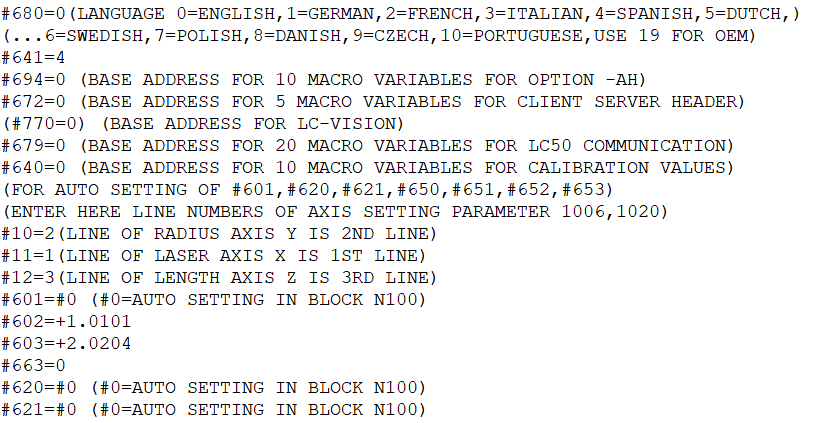
\includegraphics[scale=0.7]{pictures_and_research/Bilder/Paratab.PNG}
\caption{Auszug einer Parametertabelle}
\label{fig:Paratab}
\end{figure}
\subsection{Anforderungen}
\label{Anfs} 
An den \glqq Parametertabellenkonfigurator\grqq\space gibt es mehrere Anforderungen. \\
Parametertabellen sollen eingelesen und angezeigt werden können. Zu den Parametern soll es ermöglicht werden Beschreibungen aus Text und Bild speichern und anzeigen zu können.\\
Diese Anforderungen sind aus dem Bereich der funktionalen Anforderungen (\ref{Anforderungstypen})\\
Nicht funktionale Anforderungen (\ref{Anforderungstypen}) sind die Verwendung der Programmiersprache und das Verwenden des in C++ entwickelten Framework Qt.\\
Aus diesen Anforderungen lässt sich ableiten welche \ac{GUI}-Elemente nötig sind und welche Funktionalitäten benötigt werden.\\
Um die Anforderungen an den \glqq Parametertabellenkonfigurator\grqq\space zu sammeln, die nicht im Auftragsdokument stehen, wurde das Interview (\ref{interview}) gewählt. Die Entscheidung wurde getroffen, weil in offenen Gesprächen mehr Zusatzinformationen fließen, als in Umfragen (\ref{Fragebögen}) oder durch Beobachtung (\ref{Beobachtung}). Zusätzlich kann auf Verständnisschwierigkeiten reagiert werden, solange das Gespräch noch aktuell ist und der Kontext noch nicht vergessen ist.\\
Hauptergebnis ist die Erstellung einer übersichtlichen \ac{GUI}.\\
Die Anforderungen zielen darauf ab ein \ac{MVP} zu erstellen. Ein \ac{MVP} erfüllt die wichtigsten Anforderungen an das Produkt, ist aber noch nicht so weit entwickelt, dass es alle für den Einsatz notwendigen Anforderungen erfüllt.
\subsubsection{Notwendige Funktionalitäten}
Um die Parametertabellen anzeigen zu können müssen diese aus einer Datei eingelesen werden. Um Konfigurationen festzuhalten wird eine Funktion zum Speichern der Tabellen benötigt. \\
Für die Beschreibungen wird zusätzlich eine Funktion benötigt um diese mit den richtigen Parametern zu verknüpfen. \\
\subsubsection{Notwendige GUI-Elemente}
Die \ac{GUI} benötigt Anzeigemöglichkeiten für die Parametertabellen und Beschreibungen, Angaben von Namen, Steuerung und Produkttyp zur aktuellen Parametertabelle und den aktuellen Parameter.\\
Benötigte Steuerelemente sind Möglichkeiten um Parametertabellen und Beschreibungen zu laden und zu speichern. 
\subsection{GUI-Entwurf}
Um die \ac{GUI} zu entwerfen, kommt ein Prototyp (\ref{Prototypen}) zum Einsatz, der mit dem Mockup-Tool "Balsamiq Mockup 3\grqq\space erstellt wurde. Das Tool bietet nahezu alle gängigen \ac{GUI}-Elemente an und kann diese miteinander verknüpfen, so dass schon in einem frühen Stadium Abläufe nachvollzogen und besprochen werden können. Zusätzlich bietet das Tool eine unkomplizierte Möglichkeit alternative Entwürfe zu entwerfen und in den Ablauf der Simulation zu integrieren. Das unterstützt den Prozess während der Entwicklung der \ac{GUI}, da neue Vorschläge in kurzer Zeit besprochen und weiterentwickelt werden können.\\
\newline
Die \ac{GUI} ist aus mehreren einzelnen Fenstern aufgebaut. Dieser Aufbau unterstützt die Übersichtlichkeit und der Benutzerführung bei der Verwendung, da jeweils nur die benötigten Informationen und Funktionen angezeigt werden.\\ 
Insgesamt besteht die \ac{GUI} aus vier Fenstern, die dem Benutzer die benötigten Funktionen zur Verfügung stellen. \\
Das in Abbildung \ref{fig:filep} dargestellte Fenster dient dem Zweck bei erster Benutzung den Pfad zu einer Datenbank, in der die Beschreibungen gespeichert sind, einzugeben. Im nächsten Fenster, zu sehen in Abbildung \ref{fig:filepError}, lässt sich die Auswahl der Parametertabellen konfigurieren. Nach der Auswahl einer Parametertabelle wird diese im Hauptfenster, siehe Abbildung \ref{fig:ConfigW}, angezeigt. In diesem Fenster werden die Beschreibungen der Parameter angezeigt und die Parametertabelle kann angepasst werden. Es gibt Steuerelemente für die Navigation durch die Parametertabelle, für die Navigation durch die Fenster und die Möglichkeit die geänderte Parametertabelle zu speichern.\\
\begin{figure}[H]
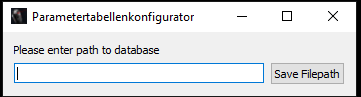
\includegraphics[scale=1]{pictures_and_research/Bilder/filepathWindow.PNG}
\caption{Fenster um den Dateipfad der Datenbank einzugeben,\\
es gibt einen Standardpfad}
\label{fig:filep}
\end{figure}
\begin{figure}[H]
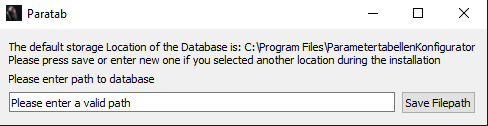
\includegraphics[scale=1]{pictures_and_research/Bilder/errorFilePathW.PNG}
\caption{Wurde ein nicht vorhandener Pfad eingegeben erscheint die Fehlermeldung "Please enter a valid path"}
\label{fig:filepError}
\end{figure}
\begin{figure}[H]
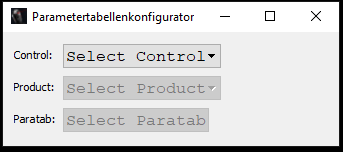
\includegraphics[scale=1]{pictures_and_research/Bilder/configW.PNG}
\caption{Fenster um Auswahl der Parametertabellen zu konfigurieren}
\label{fig:ConfigW}
\end{figure}
\begin{figure}[H]
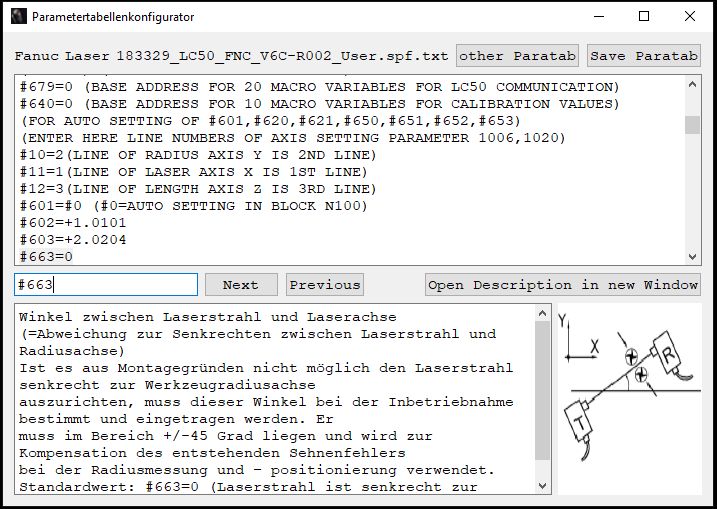
\includegraphics[scale=0.75]{pictures_and_research/Bilder/paratabW.PNG}
\caption{Fenster für die Anzeige der Parametertabellen und deren Beschreibungen}
\label{fig:Paraw}
\end{figure}
\noindent
In Abbildung \ref{fig:Paraw} werden im oberen Bereich Informationen zur aktuell ausgewählten Parametertabelle angezeigt. Oben rechts gibt es Steuerelemente um eine andere Parametertabelle auszuwählen, oder um die Aktuelle zu speichern.\\
Unterhalb der Anzeige für die Parametertabelle ist der Bereich für detaillierte Informationen zum aktuellen Parameter. Es gibt Steuerelemente um andere Parameter auszuwählen. Dies ist mit den Buttons \glqq Next\grqq\space und \glqq Previous\grqq\space möglich, die jeweils um einen Parameter nach oben oder nach unten springen. Durch direkte Eingabe eines Parameters in das Parameterfeld kann zu einem beliebigen Parameter gesprungen werden. Um größere Beschreibungen übersichtlich sehen zu können gibt es die Möglichkeit die Beschreibung isoliert in einem neuen Fenster zu öffnen.\\
\begin{figure}[H]
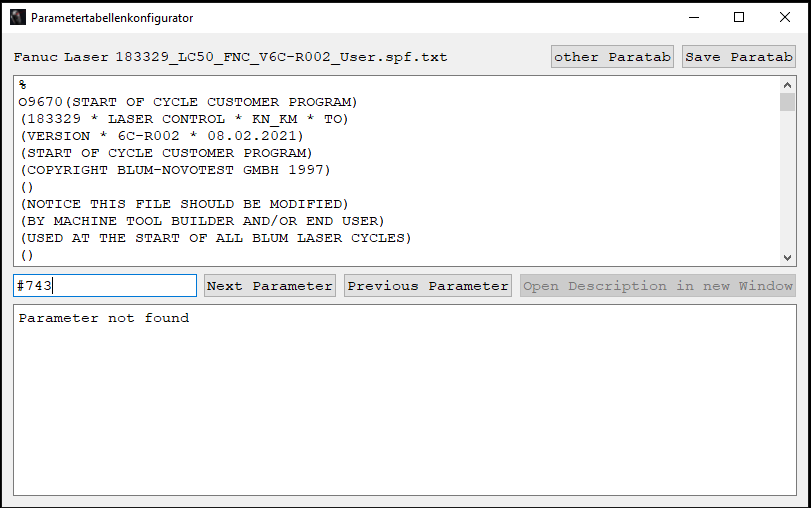
\includegraphics[scale=0.6]{pictures_and_research/Bilder/fehlermeldung_invalid_parameter.PNG}
\caption{Wird ein nicht vorhandener Parameter in das Feld eingegeben wird eine Fehlermeldung angezeigt.}
\label{fig:paraError}
\end{figure}
\begin{figure}[H]
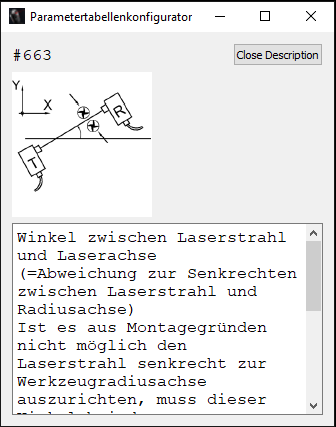
\includegraphics[scale=1]{pictures_and_research/Bilder/descriptW.PNG}
\caption{Isolierte Ansicht einer Beschreibung eines Parameters}
\label{fig:descript}
\end{figure}\noindent
Das in Abbildung \ref{fig:descript} sichtbare Bild der Beschreibung hat eine konstante Größe. Der Grund dafür ist, dass ansonsten bei Änderung der Fenstergröße das Bild verzerrt werden würde und das Erkennen von wichtigen Informationen im Bild erschwert werden würde.
\subsection{Programmierung}
Für die Programmierung wird wie in den nicht funktionalen Anforderungen (\ref{Anfs}) vorgegeben C++ mit dem für \ac{GUI} optimierten Framework Qt verwendet. \\
Da Qt für den Aufbau von Benutzeroberflächen Klassen bereitstellt, wird die Software objektorientiert (\ref{Objektorientierung}) programmiert. Um den Code auch mit wachsender Größe lesbar und verständlich zu halten kommen \lq Clean-Code Prinzipien\rq\space(\ref{CC}) zum Einsatz.\\
\subsubsection{Softwarestruktur}
Um die Software flexibel zu gestalten, wird diese mit Hilfe von modular programmiert. Die Modularität wird durch die Projektorientierte Programmierung (\ref{Objektorientierung}) unterstützt. Die Logik und die \ac{GUI} bestehen aus mehreren einzelnen Klassen, die als Module betrachtet werden können. Um die einzelnen Module zu verbinden, gibt es eine \lq Managerklasse\rq\space für den Logikteil und eine für die Module der \ac{GUI}. Um diese beiden \lq Managerklassen\rq\space ebenfalls unabhängig zu halten, gibt es eine weitere \lq Managerklasse\rq\space die dafür verantwortlich ist, die Daten zwischen Logik und \ac{GUI} zu transferieren. \\
Diese Trennung, erkennbar in Abbildung \ref{fig:UML}, ermöglicht es Anpassungen an den einzelnen Modulen vorzunehmen, ohne die höheren Ebenen grundlegend anzupassen.
\begin{figure}[H]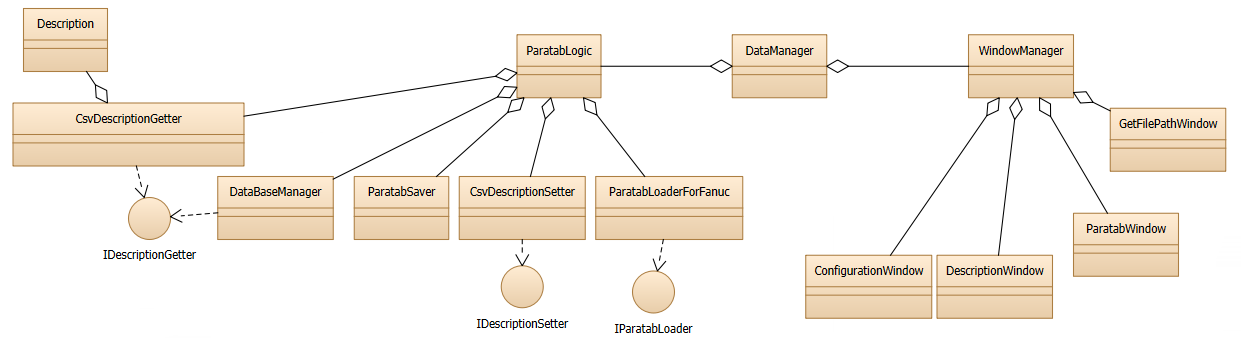
\includegraphics[page=1,scale=0.49]{pictures_and_research/Bilder/uml.PNG}
\caption{\ac{UML}-Diagramm der Software ohne attribute der Klassen}
\label{fig:UML}
\end{figure}\noindent
Das Diagramm in Abbildung \ref{fig:UML} dient dazu die Modularität der Software zu veranschaulichen, daher wurde auf die Darstellung von Inhalten der Klassen verzichtet.\\
\ac{UML} dient dazu die Architektur von Software zu visualisieren. Klassen werden durch Rechtecke visualisiert, Interfaces durch Kreise. 
\subsubsection{Verarbeitung von Benutzeraktionen}
Interagiert der Benutzer mit der \ac{GUI} werden entsprechende Veränderungen erwartet. \\
Qt bietet für die Verarbeitung der Benutzeraktionen mit dem \lq Signal-Slot Mechanismus\rq\space Unterstützung. Dieser Mechanismus bietet die Möglichkeit Signale auszusenden, die von einem verbundenen Slot empfangen werden können. Dabei muss das Senderobjekt keine Verbindung zum Empfängerobjekt haben. Die Verbindung zwischen Signal kann entweder direkt im Empfängerobjekt, oder in einer Instanz einer \lq Managerklasse\rq\space eingerichtet werden. Grundvoraussetzung ist, dass das Objekt, in dem die Verbindung eingerichtet ist, sowohl eine Verbindung mit dem Sender- als auch mit dem Empfängerobjekt hat.\\
Die meisten Klassen die von Qt bereitgestellt werden, haben vordefinierte Signale. Diese erlauben es die Benutzerinteraktionen zu verarbeiten und entsprechend darauf zu reagieren. \\
Neben den vordefinierten Signalen von \ac{GUI}-Elementen können auch selbst definierte Signale eingesetzt werden, um Methoden aufzurufen. Signale von \ac{GUI}-Elementen werden ohne weitere Implementierungen durch den Entwickler gesendet. Selbst definierte Signale müssen mit einem Befehl gesendet werden. Signale können auch Daten übergeben, die vom verbundenen Slot verarbeitet werden können. Dabei muss die Zahl der Argumente des Slots nicht mit der des Signals übereinstimmen. Signale können mit allen Slots verbunden werden, die gleich viele oder weniger Argumente entgegennehmen. Begrenzend wirkt hier die Reihenfolge der Datentypen der Argumente. Diese muss übereinstimmen.\\
Dieser Mechanismus ermöglicht weitere Flexibilität, da jederzeit neue Verbindungen erstellt werden können, oder bestehende entfernt werden können. Diese Funktionalität ist hilfreich, wenn das Ausführen einer Methode Signale aussenden würde, die unerwünschte Folgen hätten. In diesem Fall kann man die Verbindung von Signal und Slot zu Beginn der Methode trennen und am Ende der Methode wieder herstellen. \\
\subsubsection{Speicherung der Beschreibungen}
Die Beschreibungen der Parameter werden in einer relationalen Datenbank gespeichert. Relationale Datenbanken speichern Daten in Tabellen, in denen eine Spalte als eindeutiger Schlüssel , \lq Primary Key\rq\space für die Reihen dient. Relationen zwischen Elementen werden durch eine zusätzliche Spalte symbolisiert. In dieser Spalte wird der \lq Primary Key\rq\space der Reihe eingetragen, zu der eine Verbindung besteht. Es ist nicht relevant, ob die verbundene Reihe in der selben oder einer anderen Tabelle steht. In relationalen Datenbanken werden werden die Daten nicht über die Position, sondern über den \lq Primary Key\rq\space direkt adressiert. Die genaue Position der Objekte in der Datenbank ist nicht bekannt\cite{10.1145/1283920.1283937}.\\
Der Grund für die Wahl dieses Models wurde getroffen, da Beschreibungen und Bilder eindeutig einem Parameter zugeordnet werden können. Da der Parameter, für den die Beschreibung geladen werden soll, bekannt ist, ist der fehlende Zugriff über die Position kein Hindernis.
\subsubsection{Tests}
Die Software wird abgesehen von der GitLab Pipeline (\ref{Tools}) manuell getestet. Dies hat den Grund, dass die Automatisierung von Tests anspruchsvoll und zeitaufwendig ist (\ref{Tests}).
\subsubsection{Verwendete Tools}
\label{Tools}
Um die Entwicklung zu unterstützen werden Tools für die Versionsverwaltung und \lq Continous Developement/ Integration\rq\space (\ref{CI}) eingesetzt.\\
Für die Versionsverwaltung kommen GitKraken und GitLab zum Einsatz. GitKraken dient als Schnittstelle zwischen dem lokalen Projekt auf dem Computer und der Plattform für \lq Continous Developement/ Integration\rq\space \ref{CI} GitLab. In GitKraken lässt sich der gesamte Verlauf des Projekts einsehen. Außerdem können alte Commits \ref{Git} ausgewählt werden und direkt in einer Entwicklungsumgebung geöffnet werden. Für die Sicherung auf dem Server bietet GitKraken die Git Befehle, die durch eine graphische Benutzeroberfläche oder durch das integrierte Terminal genutzt werden können.\\
GitLab wird nicht nur für die Sicherung von Softwareständen auf einem Server eingesetzt. Ebenfalls genutzt werden die Möglichkeiten für das Organisieren von To-Do's durch \lq Issues\rq ,\space sowie die GitLab Pipeline. Die GitLab Pipeline ist ein Feature im Kontext von Continous Integration \ref{CI}. Zusätzlich werden während dem Prozess Artefakte erstellt, in denen Dateien gesammelt werden, die für das Erstellen eines Installers benötigt werden. Diese Artefakte lassen sich nach dem erfolgreichen Durchlauf der Pipeline als ZIP-Ordner herunterladen.\\ 
\subsection{Anwendung der Software}
Vor der Bearbeitung wird im ConfigurationWindow, Abbildung 3, die Steuerung und das Produkt festgelegt. Durch klicken auf \glqq Select Paratab\grqq\space wird ein Dateiexplorer-Fenster geöffnet. Durch die getroffene Auswahl im ConfigurationWindow, Abbildung 3, werden die angezeigten Dateien im Dateiexplorer gefiltert um die Auswahl der richtigen Parametertabelle zu vereinfachen. Die ausgewählte Parametertabelle wird im ParatabWindow, Abbildung 4 und 5, angezeigt.\\
Um einen Parameter zu bearbeiten, muss die entsprechende Zeile im Textfeld ausgewählt zu werden. Dazu gibt es unterschiedliche Möglichkeiten. Man kann eine Zeile direkt durch anklicken mit der Maus auswählen. Möchte der Benutzer jeden Parameter nacheinander konfigurieren bieten die Buttons \lq Next\rq\space und \lq Previous\rq\space die Möglichkeit direkt zum nächsten, beziehungsweise zum vorherigen Parameter zu springen, ohne danach zu suchen. Geht es darum bestimmte Parameter an verschiedenen Stellen zu bearbeiten, kann im Feld für die Anzeige des aktuellen Parameters ein Parameter eingegeben werden. Ist der eingegebene Parameter in der Tabelle enthalten, springt die Anzeige direkt zu diesem Parameter.\\
Um zu prüfen, ob eine Zeile einen Parameter enthält kommen \lq Reguläre Ausdrücke\rq\space zum Einsatz. Mit Diesen lassen sich Texte auf bestimmte Inhalte oder Muster untersuchen. \\
In dieser Software wird mit Hilfe der Cursor-Klasse von Qt die gesamte Zeile ausgewählt und mit einem \lq Regulären Ausdruck\rq\space untersucht. \\
Um die Bearbeitung der Parameter zu unterstützen wird unterhalb der Anzeige für die Parametertabelle die Beschreibung des Parameters angezeigt. Die Option \glqq Open Description in new Window\grqq ,\space Abbildung 4 und 5, hilft bei langen Beschreibungstexten und Bildern das Lesen der Beschreibung zu vereinfachen. Es öffnet sich ein neues Fenster, zu sehen in Abbildung 6, in dem die Beschreibung und das Bild isoliert angezeigt werden.\\
Ist die Konfiguration der Parametertabelle abgeschlossen, kann in der oberen rechten Ecke, zu sehen in Abbildung 4 und 5, die Parametertabelle gespeichert werden. 
% !TEX root = 4268671_Janik_Frick_T1000.tex
\section{LC-VISION}
\glqq LC-VISION\grqq\space ist eine Software von \ac{Blum} für die Visualisierung und Auswertung von Messdaten der \glqq DIGILOG-Lasermesssysteme\grqq.
Bei der Entwicklung der Software treten Unstimmigkeiten auf, die die Funktionalität der Software nicht beeinträchtigen, aber dennoch behoben werden sollten.
Während der Behebung von Unstimmigkeiten kann man von der Erfahrung anderer Entwickler profitieren. Da die Lösung in den bestehenden Code integriert wird, kommt man mit den Techniken anderer Entwickler in Kontakt. Die eigene Arbeit kann reflektiert werden\cite{34908}, wenn darüber gesprochen wird. Außerdem fördert die aktive Mitarbeit nicht nur Kenntnisse über die Theorie der Softwareentwicklung sondern auch über die praktischen Aspekte\cite{34908}.\\
Ein weiterer Vorteil ist das der Lernprozess in einer relevanten Umgebung stattfindet\cite{34908}.
Hat eine Aufgabe Relevanz kann dies einen positiven Einfluss auf die Motivation haben. \\
Bevor mit der Behebung von Unstimmigkeiten angefangen werden konnte, sollte man den Code und die Benutzeroberfläche kennenzulernen. \\
Um die Benutzeroberfläche kennenzulernen kann eine Kombination aus statischer und dynamischer Analyse verwendet werden. Bei der statischen Analyse wird nur der Code betrachtet. Um hieraus qualitative Informationen zu gewinnen, wird ein großer Teil des Codes benötigt, da nur so Zusammenhänge und Abläufe erkannt werden können\cite{mock2003dynamic}. Der Vorteil liegt darin, das dieses Verfahren auf jedem System durchgeführt werden kann, das einen Texteditor bietet. \\
In der dynamischen Analyse werden Informationen während der Laufzeit der Anwendung gesammelt. Die dynamische Analyse bringt häufig die besseren Ergebnisse, da viele Abhängigkeiten, zum Beispiel \glqq dynamic link libraries\grqq, erst zur Laufzeit eingebunden werden.
Mit diesen Analyseverfahren kann der Code optimiert werden und das Verständnis des Codes verbessert werden\cite{mock2003dynamic}.\\
Für die Einarbeitung in die Software \glqq LC-VISION\grqq\space liegt der Fokus auf der Verbesserung für das Verständnis der Abläufe. Hierzu kommt eine Kombination von statischer und dynamischer Analyse zum Einsatz. Um die obersten Schichten der Software ausfindig zu machen, wurde die dynamische Analyse genutzt. In der gestarteten Anwendung wurde nach Elementen gesucht, die im Code leicht wiederzufinden sind. Solche Elemente können Texte, Bilder oder Menüabläufe sein. Werden Muster aus der \ac{GUI} im Code gefunden kann man von dort aus Abläufen in tiefere Schichten der Software folgen. Dieser Schritt ist Teil der zuvor erwähnten statischen Analyse. Treten hierbei Probleme oder Fragen auf, kann es hilfreich sein mit einen Entwickler der Software zu sprechen, ob dieser Unterstützung bieten kann.\\
Das erworbene Wissen kann durch die Behebung von Unstimmigkeiten, wie der Anpassung von Texten und Übersetzungen, sowie inkonsistenter Datenanzeige in Sonderfällen, gefestigt werden.\\
Danach kann an Erweiterungen oder der Umstrukturierung der Software gearbeitet werden. In diesem Fall bestehen die Aufgaben aus Anpassungen und Erweiterungen der Benutzeroberfläche. Ist die Signalstärke des Lasers zu schwach, soll ein Handlungsvorschlag angezeigt werden, mit dem die Signalstärke optimiert werden kann. Eine zweite Anpassung ist eine Fehlerbehebung im Bereich der Lizenzanzeige. Informationen zu selten genutzten Lizenzen sollten nur angezeigt werden, wenn diese gekauft sind. 
\newpage
\bibliography{references}
\bibliographystyle{ieeetr}
\end{document}<div class="open_grepper_editor" title="Edit & Save To Grepper"></div>
